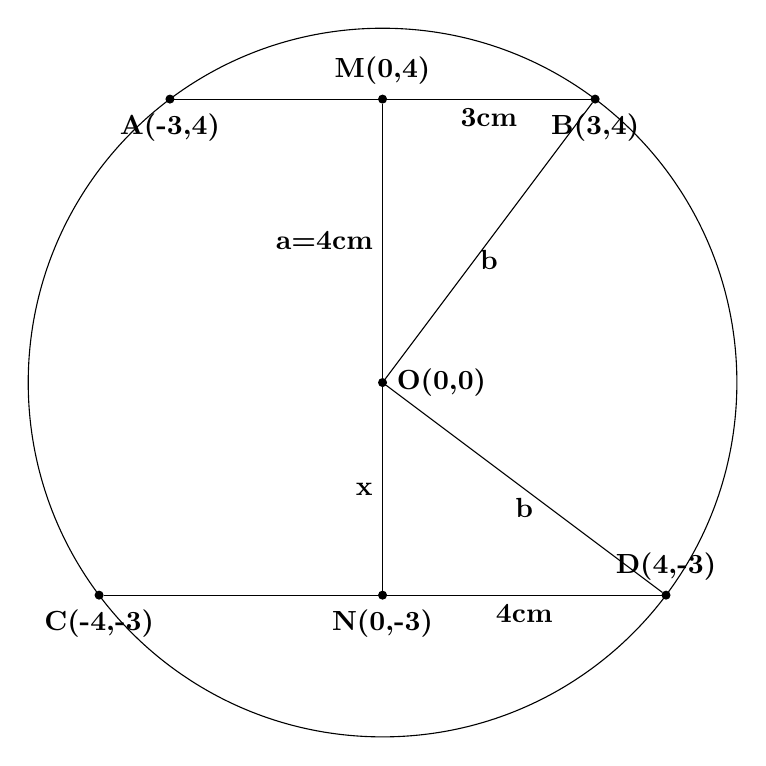
\begin{tikzpicture}[scale =0.9,>=stealth,point/.style = {draw, circle, fill = black, inner sep = 1pt},]
\draw (0,0)circle (5cm);
\node (O) at (0,0)[point,label=right :$\textbf{O(0,0)}$] {};
\node (A) at (-3,4)[point,label=below :$\textbf{A(-3,4)}$] {};
\node (B) at (3,4)[point,label=below :$\textbf{B(3,4)}$] {};
\node (C) at (-4,-3)[point,label=below :$\textbf{C(-4,-3)}$] {};
\node (D) at (4,-3)[point,label=above :$\textbf{D(4,-3)}$] {};
\node (M) at (0,4)[point,label=above :$\textbf{M(0,4)}$] {};
\node (N) at (0,-3)[point,label=below :$\textbf{N(0,-3)}$] {};
\draw (A)--(B);
\draw (C)--(D);
\draw (O)--node[left] {$\textbf{a=4cm}$}(M);
\draw (O)--node[left] {$\textbf{x}$}(N);
\draw (O)--node[below] {$\textbf{b}$}(B);
\draw (O)--node[below] {$\textbf{b}$}(D);
\draw (M)--node[below] {$\textbf{3cm}$}(B);
\draw (N)--node[below] {$\textbf{4cm}$}(D);
\end{tikzpicture}
